\documentclass[12pt,a4paper]{article}
\usepackage{geometry}
\geometry{left=2.5cm,right=2.5cm,top=2.0cm,bottom=2.5cm}
\usepackage[english]{babel}
\usepackage{amsmath,amsthm}
\usepackage{amsfonts}
\usepackage[longend,ruled,linesnumbered]{algorithm2e}
\usepackage{fancyhdr}
\usepackage{ctex}
\usepackage{array}
\usepackage{listings}
\usepackage{color}
\usepackage{graphicx}
\usepackage[hidelinks]{hyperref}
% \usepackage[colorlinks=true, linkcolor=blue, urlcolor=blue]{hyperref}  % 自訂連結顏色並移除方框
% Add the following lines
\usepackage{fontspec}
\usepackage[UTF8]{ctex}

\setmainfont{Sarasa Gothic TC}
\setCJKmainfont{Sarasa Gothic TC}
\setCJKsansfont{Sarasa Gothic TC}
\setCJKmonofont{Sarasa Gothic TC}
\begin{document}


\title{
  {
    \heiti Computer Graphics 第 3 次 Homework
  }
}


\date{
  \begin{tabular}{ll}
  2024/12/25 (聖誕節) & \hfill 
\includegraphics[width=0.06\textwidth]{img/knao-padoru.png} \\
  \end{tabular}
  }
\author{
  年級:{資工三}~~~~~~
  學號:{S11159005}~~~~~~
  姓名:{黃毓峰}~~~~~~
}


\maketitle
\newlength{\question}
\settowidth{\question}{XX}

\section*{{問題描述}}
繪製 3D 四面體(Tetrahedron),並在不同的體積分割次數(Depth)下計算並顯示其頂點數據。
為了更方便地調整分割層數,並加入物體自動旋轉控制,攝影機的操作,程式供選單可以調整。

\section*{實作/程式說明}

\noindent 新增主要功能包含:

\begin{itemize}
  \item 自動旋轉
  \item 攝影機操作
  \item 解決左右鍵功能跟 pop-menu 衝突
\end{itemize}

\subsection*{核心演算法解說}

\begin{enumerate}
  \item \textbf{自動旋轉}:
    \begin{itemize}
      \item 透過 idle 函式來實現動畫,每隔一段時間更新角度數值。
      \item 使用 glRotatef 函式,根據旋轉軸與角度來旋轉模型。
      \item 利用變數來紀錄旋轉軸、方向與角度,方便動態控制。
    \end{itemize}
    
    實作如下 (有省略部份程式):
    \newpage
    \begin{lstlisting}[language=C++,breaklines=true]
void display() {
  // ...
  if (rotationAxis == AXIS_X) {
    glRotatef(rotationAngle, 1.0f, 0.0f, 0.0f); 
  } else if (rotationAxis == AXIS_Y) {
    glRotatef(rotationAngle, 0.0f, 1.0f, 0.0f); 
  }
  else if (rotationAxis == AXIS_Z) {
    glRotatef(rotationAngle, 0.0f, 0.0f, 1.0f); 
  }
  // ...
}
  \end{lstlisting}
   

  \item \textbf{攝影機操作}:
  \begin{itemize}
    \item 使用球座標系統來控制攝影機的位置。
    \item 透過滑鼠的拖曳動作來改變球座標的參數 (角度與距離)。
    \item 使用 gluLookAt 函數來設定攝影機的視角。
  \end{itemize}
  
  實作如下 (有省略部份程式):
  \newline
  \begin{lstlisting}[language=C++,breaklines=true]
void display() {
  // ...
  float cX = radius * sinf(phi) * cosf(theta);
  float cY = radius * cosf(phi);
  float cZ = radius * sinf(phi) * sinf(theta);

  gluLookAt(cX, cY, cZ,    
            0.0f, 0.0f, 0.0f,   
            0.0f, 1.f, 0.0f);  
  // ...
}
\end{lstlisting}
\newpage
\begin{lstlisting}[language=C++,breaklines=true]
void mouseMotion(int x, int y) {
    int dx = x - prevMouseX;
    int dy = y - prevMouseY;

    if(
      (mouseButtonPressed & (1 << GLUT_LEFT_BUTTON)) != 0 &&
      (mouseButtonPressed & (1 << GLUT_RIGHT_BUTTON)) == 0
    ) 
    {
        theta += dx * 0.005f; 
        phi   -= dy * 0.005f;

        if(phi <= 0.01f) phi = 0.01f;
        if(phi >= 3.13f) phi = 3.13f;
    }

    if(
      (mouseButtonPressed & (1 << GLUT_LEFT_BUTTON)) != 0 &&
      (mouseButtonPressed & (1 << GLUT_RIGHT_BUTTON)) != 0
    ) 
    {
      radius += dy * 0.01f;

      if(radius < 1.0f) radius = 1.0f;
      if(radius > 10.0f) radius = 10.0f;
    }

    prevMouseX = x;
    prevMouseY = y;

    glutPostRedisplay(); 
}

  \end{lstlisting}
  \newpage
  \item \textbf{解決左右鍵功能跟 pop-menu 衝突}:
    要解決這個問題,我們需要在程式碼中加入額外的判斷,確保在左右鍵同時被按下的時候,不要觸發右鍵的彈出式選單。
    
    具體做法是,在左鍵被按下時,先暫時取消右鍵的選單功能,在放開左鍵時,再將右鍵選單恢復。
    
    實作如下 (有省略部份程式):
    \begin{lstlisting}[language=C++,breaklines=true]
void mouseButton(int button, int state, int x, int y) {
  prevMouseX = x;
  if(state == GLUT_DOWN) {
      // Set the bit corresponding to the pressed button
      mouseButtonPressed |= 1 << button;
      prevMouseY = y;
      glutDetachMenu(GLUT_RIGHT_BUTTON);
  } else if(state == GLUT_UP) {
      // Clear the bit corresponding to the released button
      mouseButtonPressed &= ~(1 << button);
      glutAttachMenu(GLUT_RIGHT_BUTTON);
  }
}
  \end{lstlisting}


\end{enumerate}
\newpage
\subsection*{程式架構}
\noindent 主要函數說明:
\begin{itemize}
\item \texttt{tetrahedron}:遞迴實現四面體細分
\item \texttt{draw\_triangle\_3d}:繪製四面體的四個面
\item \texttt{midpoint}:計算兩點的中點
\item \texttt{mouseButton}:處理滑鼠按鍵事件
\item \texttt{mouseMotion}:處理滑鼠移動事件
\item \texttt{idle}:用於動畫效果,定期更新旋轉角度
\item \texttt{display}:繪製場景,包含模型與攝影機設定
\item \texttt{processAxisMenu}:處理選單中選擇旋轉軸的事件
\item \texttt{processDirectionMenu}:處理選單中選擇旋轉方向的事件
\item \texttt{createMenu}:建立互動選單
\end{itemize}

\section*{程式編譯環境}
\subsection*{電腦軟體系統簡介}
\begin{itemize}
  \item Linux 6.11.5
  \item gcc - 14.2.1
  \item cmake - 3.30.5
  \item Wayland
  \item OpenGL - 4.6 
\end{itemize}



\subsection*{GLFW函式庫名稱與版本}

\begin{itemize}
  \item freeglut - 3.6.0-2 
\end{itemize}
\newpage
\section*{編譯後的執行成果}
\begin{figure}[h]
  \centering
  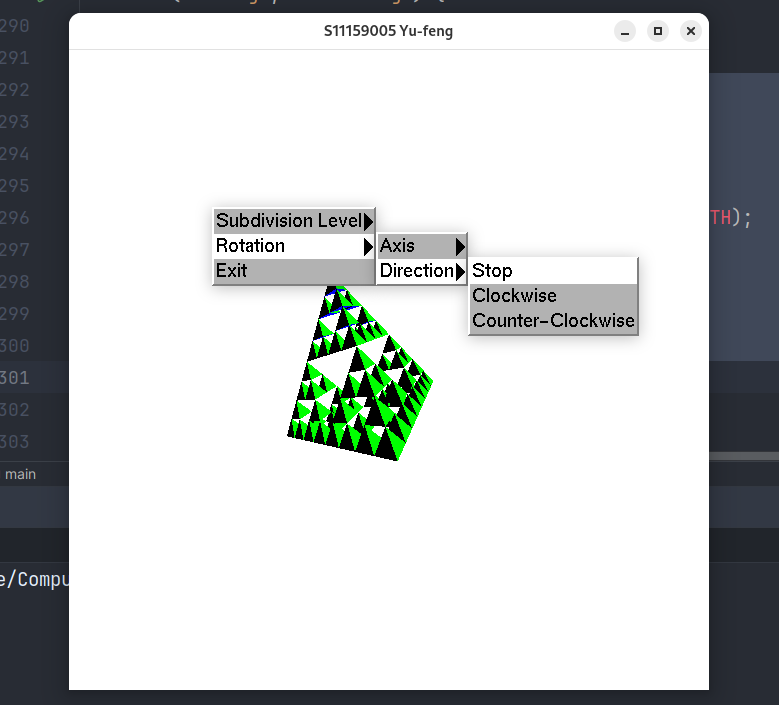
\includegraphics[width=0.8\textwidth]{img/hw3_result.png}
  \caption{執行結果}
\end{figure}

\section*{心得}
在這次的作業中,我學到了一件事有時候時間不夠就不要硬要手刻一些功能(pop-menu),
也就是我從 glfw 改用 freeglut ,還有複習了我的數學以及學到更多圖學知識。

\section*{SourceCode}
\sloppy
\noindent \url{https://github.com/IDK-Silver/NUTN-CSIE-Code/tree/main/ComputerGraphics/hw3}




\end{document}
